% Compact PGFPlots panel for sampled qldpc_96_4_7_fixed_k_absorb_cap7 BSC correction-class derivative.
% Requires \usepackage{pgfplots} and \pgfplotsset{compat=1.18}.
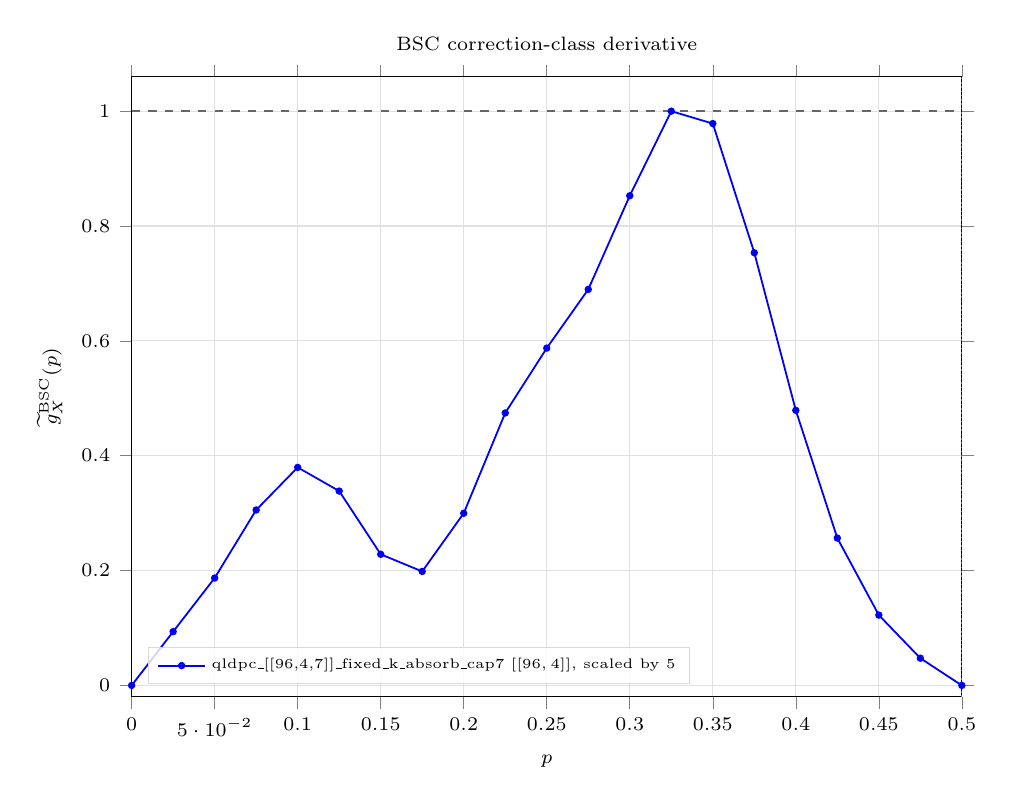
\begin{tikzpicture}
\begin{axis}[
  name=scaledBSCGEXITQldpc9647FixedKAbsorbCap7Axis,
  width=\linewidth,
  height=0.78\linewidth,
  title={BSC correction-class derivative},
  title style={font=\scriptsize},
  xlabel={$p$},
  ylabel={$\widetilde g_X^{\rm BSC}(p)$},
  xmin=0, xmax=0.5,
  ymin=-0.02, ymax=1.06,
  grid=both,
  major grid style={black!12},
  minor grid style={black!6},
  tick align=outside,
  tick label style={font=\scriptsize},
  label style={font=\scriptsize},
  legend cell align={left},
  legend style={draw=black!15, fill=white, fill opacity=0.82, text opacity=1, at={(0.02,0.02)}, anchor=south west, font=\tiny},
]
\addplot[black!60, densely dotted, line width=0.55pt, forget plot] coordinates {(0.5,-0.02) (0.5,1.06)};
\addplot[black!60, dashed, line width=0.55pt, forget plot] coordinates {(0,1) (0.5,1)};
\addplot+[color=blue, mark=*, mark size=1.0pt, line width=0.65pt]
coordinates {(0,0) (0.025,0.0936566104854) (0.05,0.187060981657) (0.075,0.305563789664) (0.1,0.379656417621) (0.125,0.338466661739) (0.15,0.228340249735) (0.175,0.198466278811) (0.2,0.299809544046) (0.225,0.474460140871) (0.25,0.587400888874) (0.275,0.689632176431) (0.3,0.852750595267) (0.325,1) (0.35,0.978438026395) (0.375,0.753469441775) (0.4,0.47904564294) (0.425,0.256573692776) (0.45,0.122476781462) (0.475,0.0473863416995) (0.5,0)};
\addlegendentry{qldpc\_[[96,4,7]]\_fixed\_k\_absorb\_cap7 $[[96,4]]$, scaled by $5$}
\end{axis}
\end{tikzpicture}
